\documentclass[11pt]{article}

\usepackage[utf8]{inputenc}
\usepackage[T1]{fontenc}
\usepackage[margin=1in]{geometry}
\usepackage{amsmath}
\usepackage{booktabs}
\usepackage{graphicx}
\usepackage{xcolor}
\usepackage{enumitem}
\usepackage[colorlinks=true,linkcolor=blue,urlcolor=blue]{hyperref}

\definecolor{leakred}{HTML}{C44E52}
\definecolor{okgreen}{HTML}{55A868}
\definecolor{ctrlblue}{HTML}{4C72B0}

\graphicspath{{./}}

\newcommand{\tabst}{|t|}
\newcommand{\code}[1]{\texttt{#1}}

\title{Results summary}
\author{}
\date{}

\begin{document}
\maketitle


\hrulefill

\section{Method of detection}



\begin{enumerate}[leftmargin=1.4em]
  \item \textbf{Fault model}  instruction skip: step the PC past a \code{bl},
    so that one operation never executes. Applied to all 20 operation-calls in
    the signing loop, one at a time.
  \item \textbf{Feature}  the \textbf{matched filter}:  correlation
    of the sparse challenge $c$ against each response polynomial $z$ (a
    1024-vector, $L=4$ polys $\times$ 256 lags). The \emph{marginal} of $z$ is
    secret-independent by design, so a plain histogram of $z$ is blind; the leak
    lives only in the joint $(c, z)$.
  \item \textbf{Verdict, two equivalent ways:}
  \begin{itemize}
    \item \textbf{Two-key classifier accuracy} (leave-one-out). Signed score
      $\mathrm{score}(x) = \langle x, g_{\text{own}}^{\text{LOO}}\rangle -
      \langle x, g_{\text{other}}\rangle$ against per-key mean templates; key-A
      sigs should score $>0$, key-B $<0$. 50\% = indistinguishable, 100\% =
      leak, flag at $\ge 80\%$.
    \item \textbf{TVLA t-test} (\code{ttest\_09.py}). Welch two-sample $t$ at
      every one of the 1024 matched-filter coordinates between key A and key B;
      flag any coordinate with $\tabst > 4.5$ ($\approx p < 10^{-5}$). 
  \end{itemize}
\end{enumerate}

The two verdicts agree on every site.

\hrulefill

\section{Positive result}

\begin{table}[h]
\centering
\begin{tabular}{@{}llccccc@{}}
\toprule
site & addr & two-key acc & TVLA $\max\tabst$ & \#coords $>4.5$ & perm $p$ \\
\midrule
\textbf{\code{z = z + y} (polyvecl\_add)} & \code{0x4d5e} & \textbf{100\%} &
\textbf{15.4} & \textbf{444 / 1024} & \textbf{0.0005} (floor) \\
\bottomrule
\end{tabular}
\end{table}



\section{Negative results}

Two distinct kinds of non-leak.

\subsection{(a) Runs fine, but no leak}

Nine sites complete signing yet stay at chance. The mask survives (or the
skipped step doesn't touch it), so key A and key B overlap on the decision
boundary.

\begin{table}[h]
\centering
\begin{tabular}{@{}llcccc@{}}
\toprule
site & addr & acc (N=16) & acc (N=28) & TVLA $\max\tabst$ & \#coords $>4.5$ \\
\midrule
control (no fault) & --- & 53\% & 52\% & 3.6 & 0 \\
memcpy & \code{0x4c90} & 47\% & 46\% & 3.6 & 0 \\
$y \to$ NTT & \code{0x4c9a} & 41\% & 50\% & 3.6 & 0 \\
$w = A\cdot y$ & \code{0x4cb0} & 41\% & 54\% & 3.4 & 0 \\
$w \to$ invNTT & \code{0x4cc4} & 75\% & 46\% & 3.9 & 0 \\
pack $w_1$ & \code{0x4cec} & 69\% & 50\% & 3.7 & 0 \\
shake squeeze $\tilde{c}$ & \code{0x4d18} & 47\% & \emph{(hang at N=28)} & --- & --- \\
reduce $z$ & \code{0x4d68} & 38\% & 46\% & 3.5 & 0 \\
pack $z$ into sig & \code{0x4d88} & 41\% & 59\% & 3.3 & 0 \\
$w_0 - c\cdot s_2$ & \code{0x4dca} & 59\% & 59\% & 3.6 & 0 \\
\bottomrule
\end{tabular}
\end{table}

% \noindent\textbf{Robustness note.} At the sweep's N=16, two sites drifted up ---
% $w \to$ invNTT (75\%) and pack $w_1$ (69\%) --- close to the 80\% line. At N=28
% they fall back to 46\% / 50\% with \textbf{zero} TVLA coordinates over threshold.
% That is the safeguard working: the accuracy wobble is small-sample noise, and the
% direction-free TVLA test refuses to confirm any of them. The non-leak sites all
% sit at $\max\tabst \approx 3.3\text{--}3.9$ --- the noise ceiling for the largest
% of 1024 near-null t-values, and the same number the t-test gives on the
% \textbf{raw z} coefficients ($\max\tabst \approx 3.4$, blind). Only $z=z+y$
% breaks out of that band.

\subsection{(b) Hangs because the skip breaks the loop}

Since Signing is reject-and-retry; a
whole-call skip drops a value a rejection check depends on, the check fails every
iteration, and the loop never accepts.

\begin{quote}
\code{sample y} $\cdot$ \code{decompose w} $\cdot$ \code{poly\_challenge}
$\cdot$ \code{c*s1} $\cdot$ \code{z-norm check} $\cdot$ \code{c*s2} $\cdot$
\code{r0 check} $\cdot$ \code{c*t0} $\cdot$ \code{ct0 check} $\cdot$
\code{make\_hint}
\end{quote}

\noindent\textbf{The important negative:} the three \textbf{rejection-check}
skips (\code{z-norm}, \code{r0}, \code{ct0}) hang rather than leak, even
though those checks \emph{are} the zero-knowledge mask and faulting them
\textbf{does} leak. The reason is that a whole-call skip breaks the loop because the next check sees a stale value, and the loop never accepts

\begin{table}[h]
\centering
\begin{tabular}{@{}llll@{}}
\toprule
 & fault model & effect & outcome \\
\midrule
this sweep & skip the whole \code{bl poly\_chknorm} & $r_0$ = stale $\neq 0 \to$
always \textbf{reject} & hang \\
The paper & force the \code{cmp} result to 0 & $r_0 = 0 \to$ always
\textbf{accept} & leak \\
\bottomrule
\end{tabular}
\end{table}

% \noindent A whole-call skip breaks the loop in the wrong direction to
% expose the check-bypass leak; that leak needs example 08's targeted
% stuck-at-accept fault and a lattice/polytope solver over many signatures --- a
% different fault class and heavier analysis than a per-signature two-key
% distinguisher. This sweep also does not rediscover \textbf{category 4.1}
% (partial-nonce loop-abort), which a whole-call skip cannot express.


\section{Plots}

\begin{figure}[h]
\centering
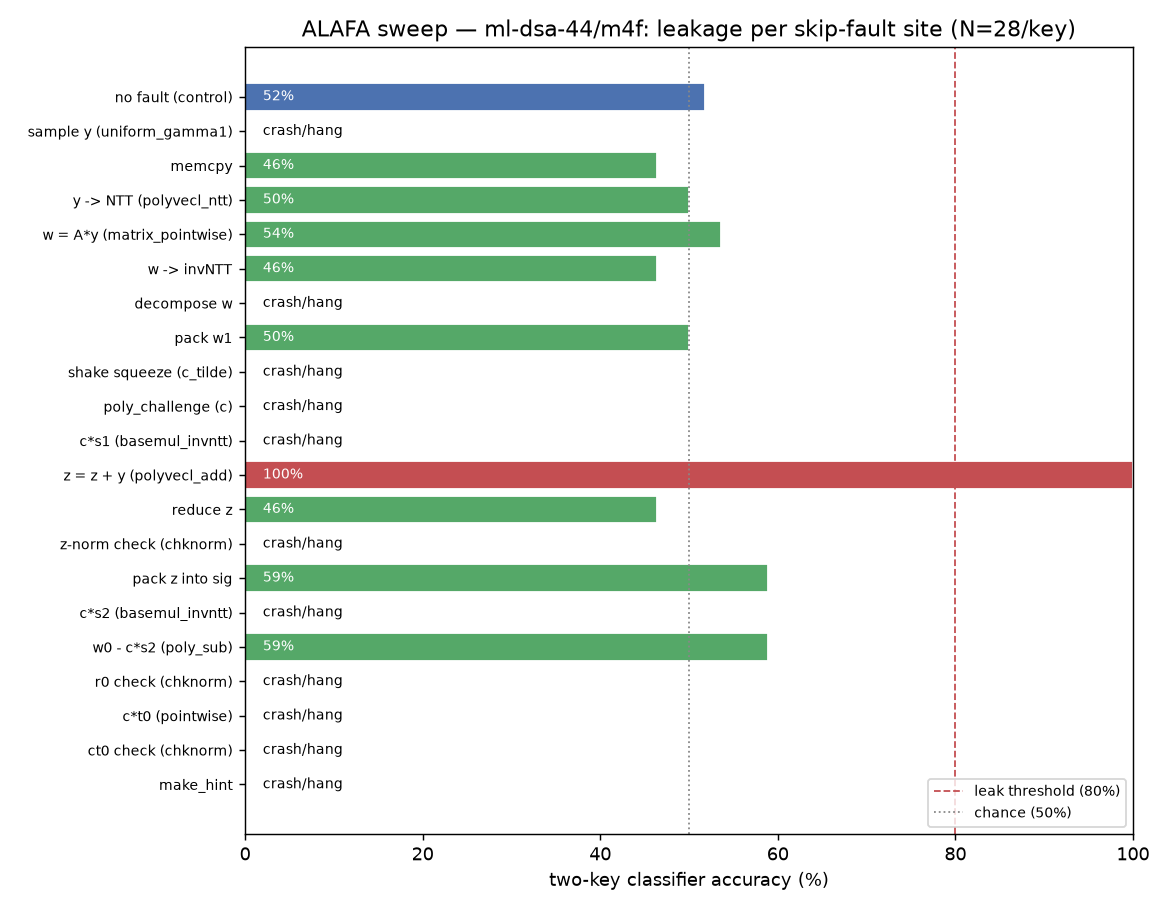
\includegraphics[width=0.86\textwidth]{alafa_accuracy.png}
\caption{Two-key classifier accuracy per fault site. Blue = control, red = leak,
green = ran/no leak, grey = hang. Dashed line = 80\% leak threshold, dotted =
50\% chance.}
\end{figure}

\begin{figure}[h]
\centering
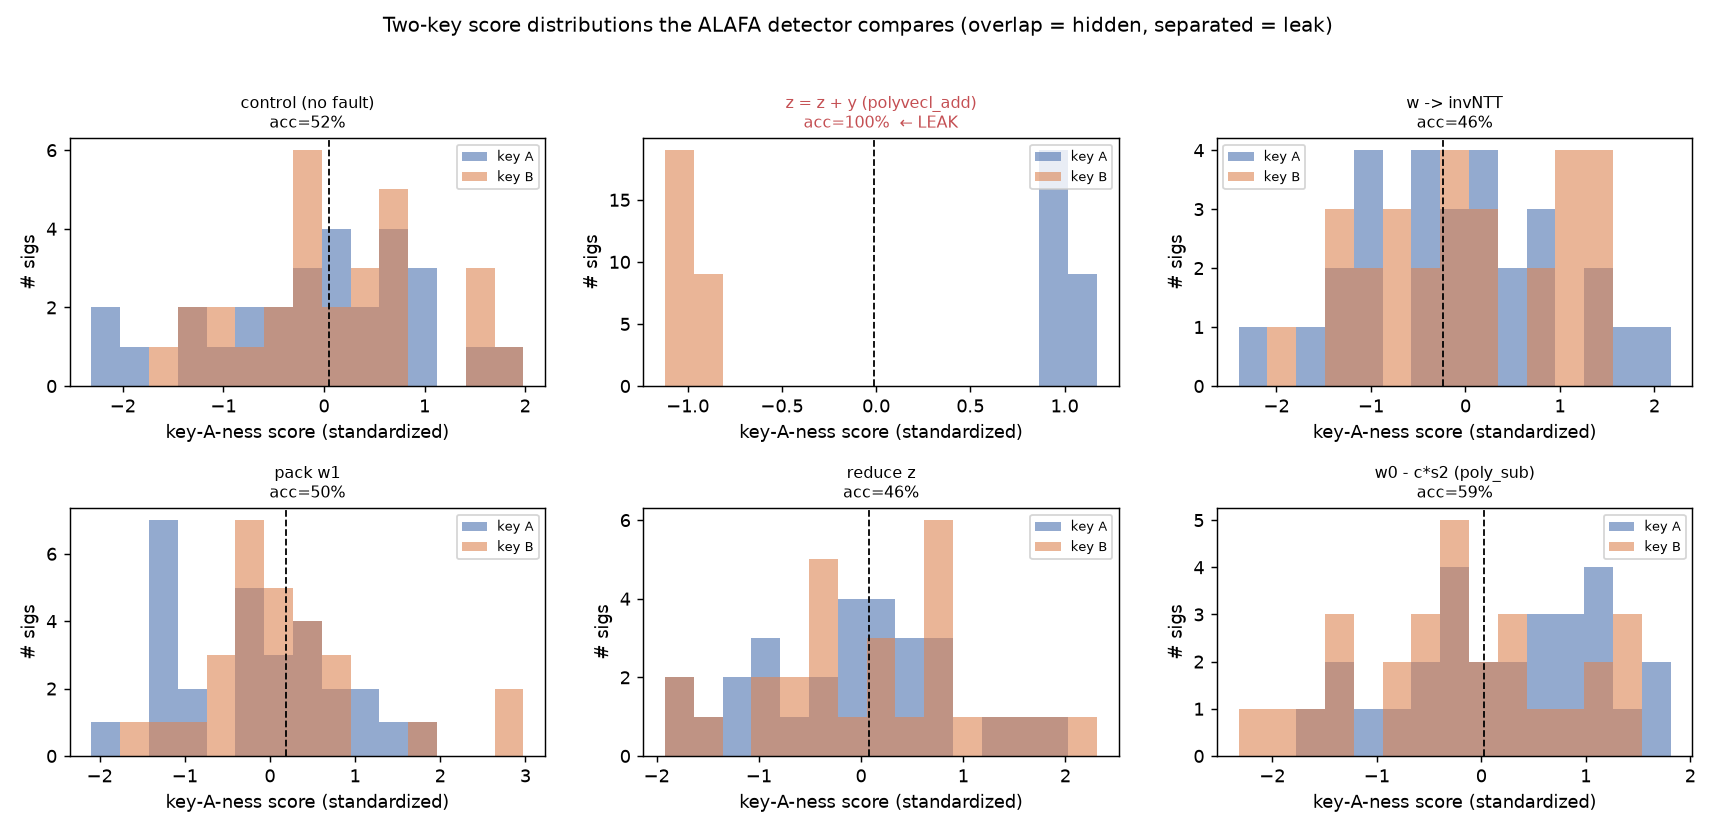
\includegraphics[width=\textwidth]{distributions.png}
\caption{Two-key score distributions at representative sites. Overlap = the
output hides the key; separated = leak. Only $z=z+y$ separates.}
\end{figure}

\begin{figure}[h]
\centering
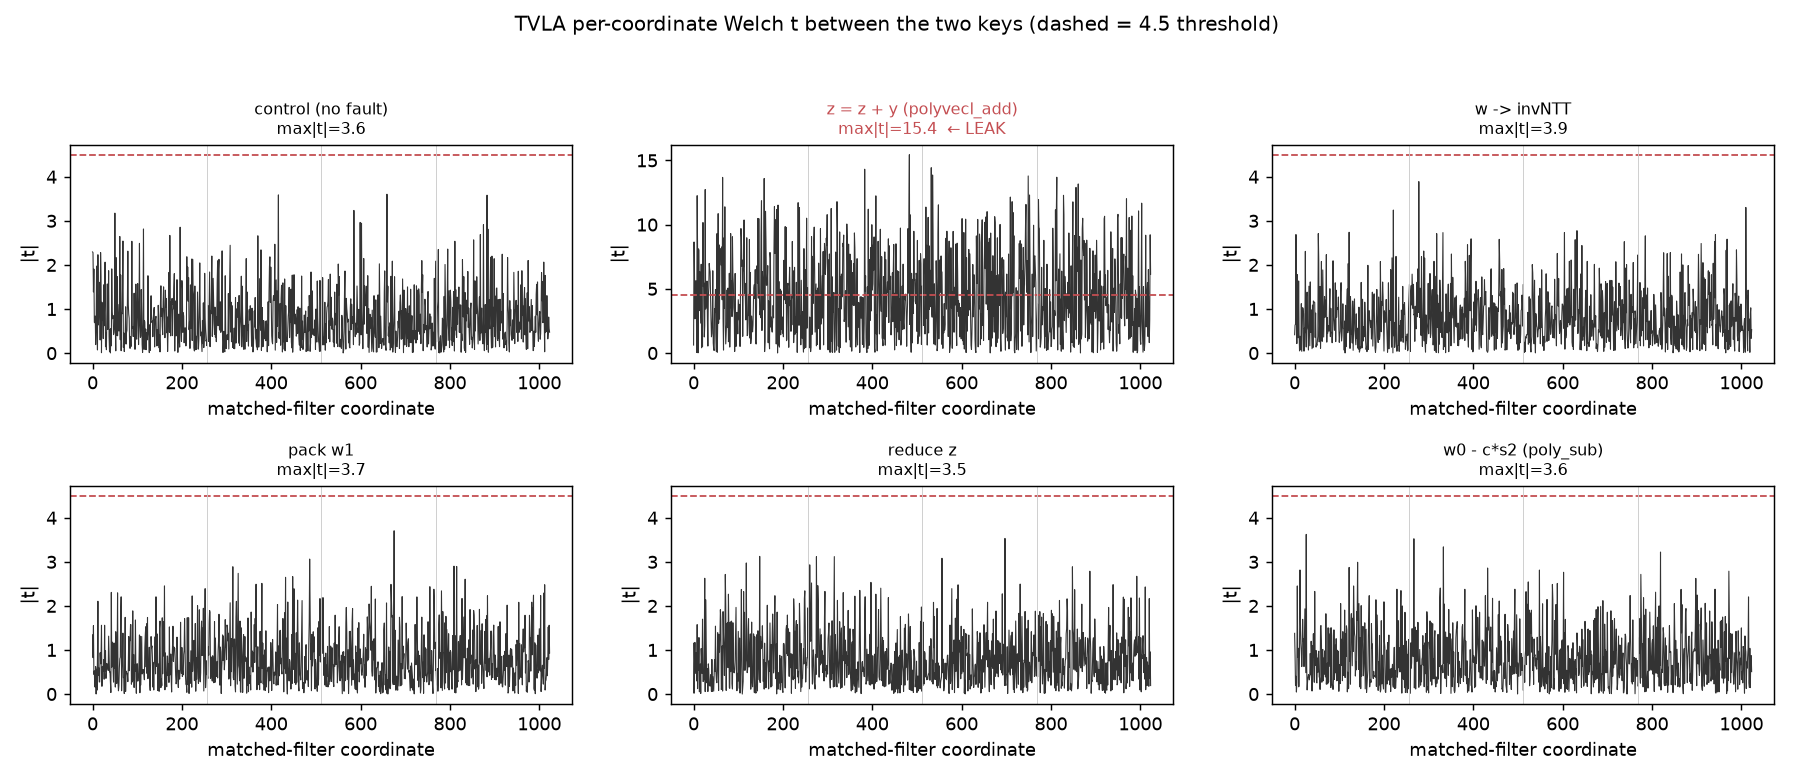
\includegraphics[width=\textwidth]{tvla_trace.png}
\caption{Per-coordinate $\tabst$ across the 1024 matched-filter features, one
panel per representative site, with the $4.5$ threshold dashed. Non-leak sites
hug the bottom; only $z=z+y$ is lifted bodily above the line.}
\end{figure}

\begin{figure}[h]
\centering
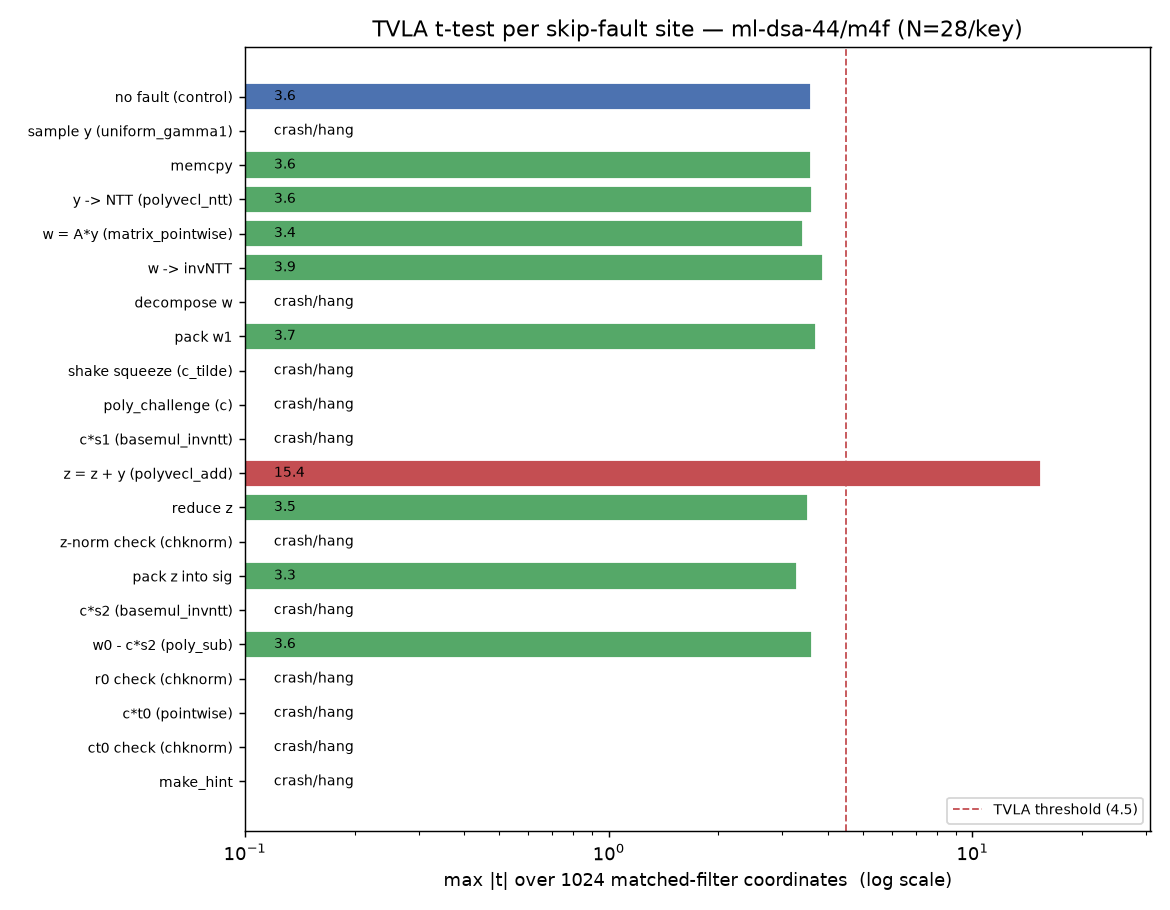
\includegraphics[width=\textwidth]{tvla_maxt.png}
\caption{$\max\tabst$ per fault site (log scale), with the $4.5$ threshold }
\end{figure}

% \begin{table}[h]
% \centering
% \begin{tabular}{@{}ll@{}}
% \toprule
% file & shows \\
% \midrule
% \code{alafa\_accuracy.png} & two-key accuracy per site (colour-coded) \\
% \code{distributions.png} & two-key score histograms --- overlap vs separated \\
% \code{score\_<site>.png} & the six representative panels, standalone \\
% \code{tvla\_trace.png} & per-coordinate $\tabst$ across the 1024 features \\
% \code{tvla\_maxt.png} & $\max\tabst$ per site (log scale) \\
% \bottomrule
% \end{tabular}
% \end{table}

% \section{Reproducing}

% \begin{verbatim}
% .venv/bin/python examples/09_alafa_sweep.py    # ASCII sweep  (N=16/key)
% .venv/bin/python examples/plots/plot_09.py     # distribution plots (N=28/key)
% .venv/bin/python examples/plots/ttest_09.py    # t-test table + plots (N=28/key)
% .venv/bin/python examples/plots/diag_crash.py  # hang-vs-crash diagnosis
% \end{verbatim}

\end{document}
